\begin{frame}
  \frametitle{Infinite multiplication factor for unit cell model}
    \begin{columns}
    \column[t]{7cm}
   \vspace{-0.35in}
  \begin{figure}[t]
   \hspace*{-0.2in}
   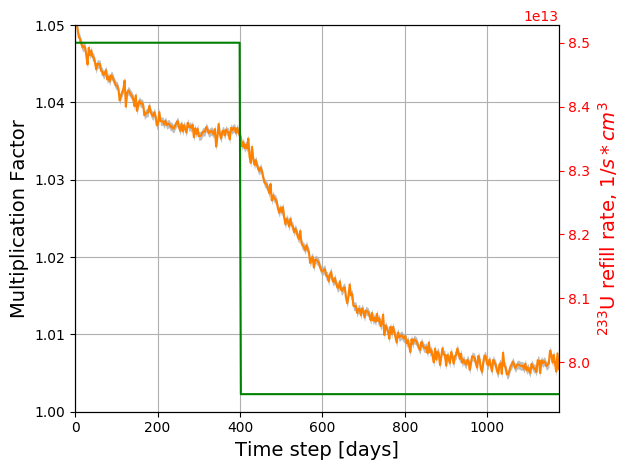
\includegraphics[height=0.75\textheight]{./images/keff.png}
   \vspace{-0.05in}
   \caption{Infinite multiplication factor during a 1200 days depletion simulation. The confidence interval $\pm\sigma$ is shaded.}
    \end{figure}

    \column[t]{4.5cm}
       \begin{itemize}
        \item Strong absorbers ($^{233}$Th,$^{234}$U) accumulating in the begining of cycle. 
   		\item Fissile materials other than $^{233}$U producing in the core ($^{235}$U, $^{239}$Pu).
   		\item Fresh fuel refill rate was changed after 400 days of operation to adjust this effects.
   		\item The multiplication factor stabilizes after approximately 950 days.
       \end{itemize}
     \end{columns}
\end{frame}

\begin{frame}
  \frametitle{Fuel salt composition evolution}
    \begin{columns}
    \column[t]{7cm}
   \vspace{-0.35in}
  \begin{figure}[t]
   \hspace*{-0.15in}
   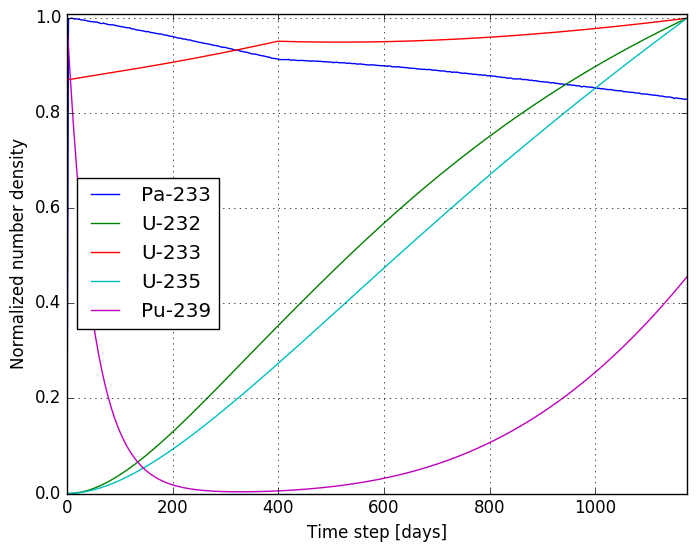
\includegraphics[height=0.75\textheight]{./images/fuel_composition.png}
   \vspace{-0.05in}
   \caption{Normalized number density of major isotopes during 1200 days of depletion.}
    \end{figure}

    \column[t]{5cm}
       \begin{itemize}
        \item Number density of $^{233}$Pa is negligible (10$^{16}$ 1/cm$^3$) but some small amount of it is produced
during the 3-day reprocessing period. 
   		\item Fissile materials other than $^{233}$U producing in the core ($^{235}$U, $^{239}$Pu).
   		\item $^{239}$Pu from initial fissile loading fully depleted after 250 days but then slowly producing from $^{238}$U.
       \end{itemize}
     \end{columns}
\end{frame}

\begin{frame}
  \frametitle{Rate of change $^{232}$Th and $^{233}$U in the core}
    \begin{columns}
    \column[t]{7.5cm}
   \vspace{-0.35in}
  \begin{figure}[t]
   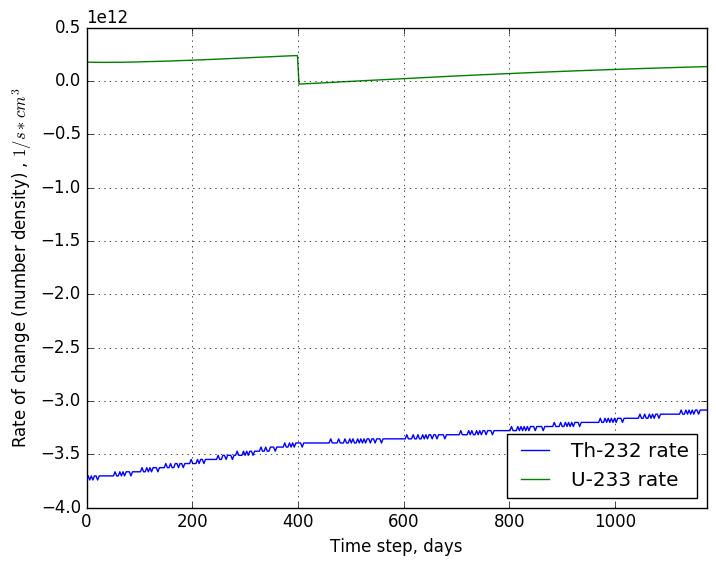
\includegraphics[height=0.75\textheight]{./images/rates_fuel.png}
   \vspace{-0.05in}
   \caption{Major isotopes rate of change during online reprocessing.}
    \end{figure}

    \column[t]{4.5cm}
       \begin{itemize}
        \item To keep the reactor critical, a higher $^{233}$U flow rate from the protactinium decay tank required for
the first 400 days.
   		\item The $^{232}$Th rate of loss slightly decreases over 4 years of operation due to fissile materials accumulation.
       \end{itemize}
     \end{columns}
\end{frame}

\begin{frame}
  \frametitle{Rate of change $^{233}$Pa, $^{233}$U from the protactinium decay tank}
    \begin{columns}
    \column[t]{8cm}
   \vspace{-0.35in}
  \begin{figure}[t]
   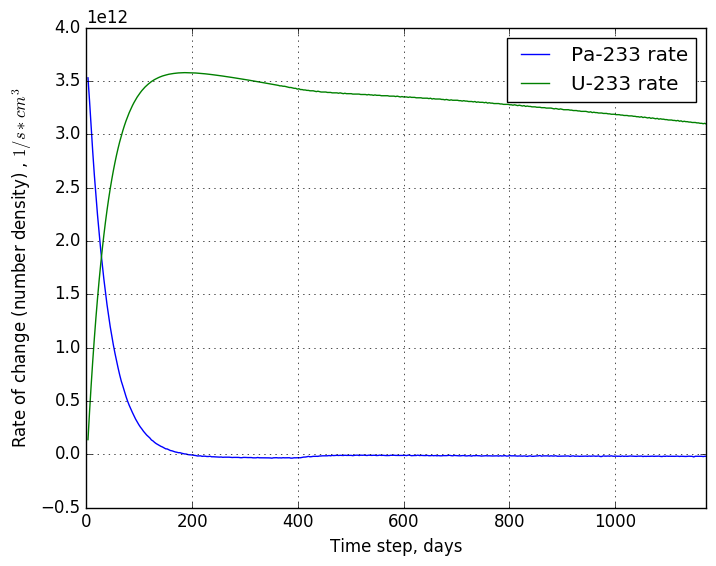
\includegraphics[height=0.8\textheight]{./images/rates_outflow.png}
   \vspace{-0.12in}
   \caption{Isotopes rate of change for the protactinium decay tank during MSBR online reprocessing.}
    \end{figure}

    \column[t]{4cm}
        \begin{itemize}
        \item Protactinium accumulated for approximately 200 days.
   		\item Fresh fissile $^{233}$U fuel flow established after 200 days.
   	  \end{itemize}
     \end{columns}
\end{frame}

\begin{frame}
  \frametitle{Neutron spectrum}
   \vspace{-0.5in}
  \begin{figure}[t]
   \hspace*{-0.39in}
   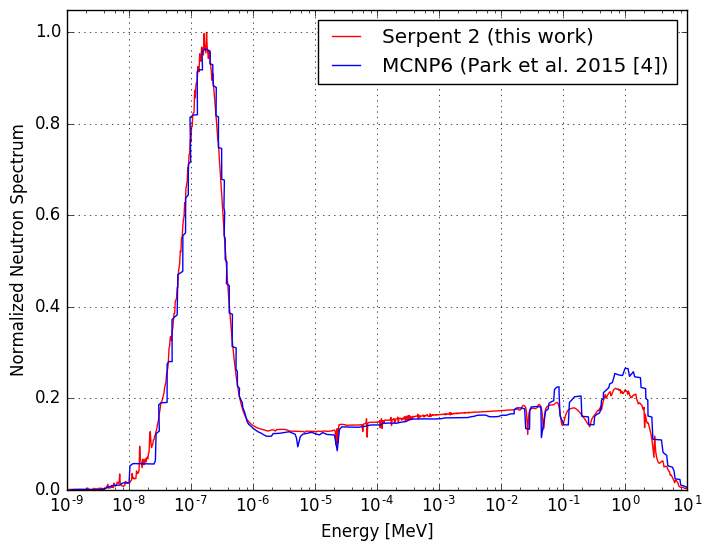
\includegraphics[height=0.8\textheight]{./images/spectrum.png}
   \vspace{-0.1in}
   \caption{Neutron spectrum for initial and equilibrium composition (normalized per lethargy).}
    \end{figure}
    \vspace{-0.1in}
    \begin{itemize}
       \item \gls{MSBR} has a epithermal spectrum which is perfect for thorium fuel cycle.
       \item Spectrum becames harder due to heavy fission products accumulation.
    \end{itemize}   
\end{frame}

